\chapter{EKSPERIMEN NUMERIK}
% Percobaan numerik yang dilakukan pada bab ini bertujuan untuk mengamati tingkat akurasi, sifat monoton dari interpolasi dengan menggunakan metode pendekatan numerik pada turunan pertama yang berbeda sebagaimana yang telah dibahas pada bab sebelumnya. Dengan mengamati properti dari hasil interpolasi tersebut kita dapat menyimpulkan kelebihan dan kekurangan dari setiap metode yang digunakan.

Pada bab ini akan dilakukan eksperimen numerik untuk mengamati tingkat akurasi dari metode numerik yang telah dibahas pada bab sebelumnya. Eksperimen dilakukan dengan menggunakan bahasa pemrograman $Python$. Setiap eksperimen dilakukan untuk mengamati tingkat akurasi metode pada kondisi tertentu.

Terdapat tiga buah eksperimen yang akan dilakukan dengan menggunakan tiga buah metode yang sudah didefinisikan sebelumnya berupa

\begin{tabular}{cp{10.5cm}}
  $\textbf{S}$  :& Interpolasi spline kubik dengan kondisi batas $S'(a) = f'(a)$ dan $S'(b) = f'(b)$.\\
  $\textbf{R}_k$  :& Metode interpolasi spline kubik monoton dengan regularitas maksimum yang dibahas pada Bagian \ref{4.2}.\\
  $\textbf{O}_k$  :& Metode interpolasi spline kubik monoton dengan order akurasi maksimum yang dibahas pada Bagian \ref{4.3}.\\
\end{tabular}\\
Pada metode $\textbf{R}_k$ dan $\textbf{O}_k$, notasi $k$ menotasikan pendekatan nilai turunan pertama yang digunakan, dengan $k = FB,~AY$ merupakan metode yang didefinisikan pada Persamaan \eqref{dotf_FB} dan Persamaan \eqref{dotf_AY} secara berurutan.

Dalam melakukan estimasi tingkat order akurasi didefinisikan
\begin{align*}
    o_l^W := \log_2(\frac{e_l^W}{e_{l-1}^W}),
\end{align*}
dengan $W$ adalah himpunan indeks yang diamati nilai galatnya serta
\begin{align*}
    e_l^W := \max_{i \in W} |f'(x_i) - \dot{f}_i|.
\end{align*}

\section{Eksperimen Pertama}

Pada eksperimen pertama diberikan fungsi
\begin{align*}
    f(x) = x^4 + \sin(x),
\end{align*}
pada interval $[0,2]$ sebagai fungsi yang akan diinterpolasikan. Dalam eksperimen ini interval akan dibagi menjadi beberapa subinterval yang sama besar dan subinterval yang tidak sama besar.

\begin{figure}[htp]
    \centering
    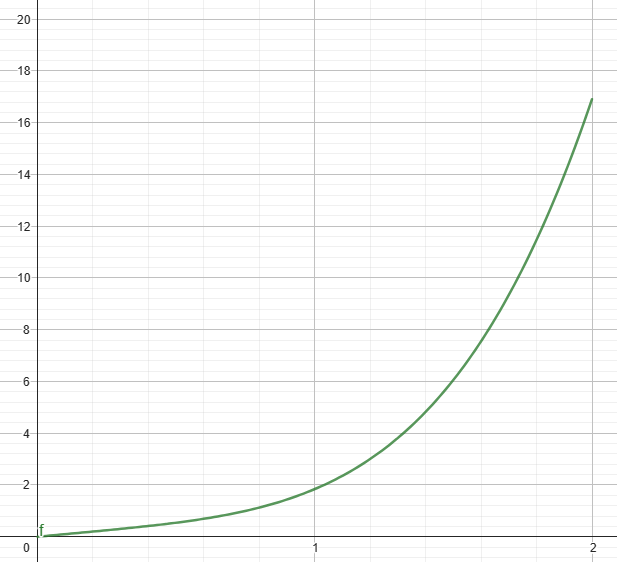
\includegraphics[width=7cm]{Images/figure_2/percobaanSatu.png}
    \caption{Grafik fungsi $f$ pada eksperimen pertama}
    \label{grafikf1}
\end{figure}

Dari Gambar \ref{grafikf1} diperoleh fungsi $f$ merupakan fungsi yang kontinu pada interval $[0,2]$. Eksperimen dengan menginterpolasi titik pada fungsi $f$, dilakukan untuk mengamati tingkat akurasi metode ketika menginterpolasi fungsi kontinu.
\subsection{Interval Sama Besar}

Untuk membagi interval $[0,2]$ menjadi beberapa interval sama besar dibentuk titik-titik $x_j^l = j/2^l, ~ j=0,\dots,2^{l+1}$, dengan $l$ suatu bilangan bulat positif. Dari titik-titik tersebut dibentuk subinterval-subinterval pada interval $[0,2]$ berupa $[x_j^l, x_{j+1}^l], ~ j=0,\dots,2^{l+1}-1$. Pada setiap interval tersebut akan dilakukan interpolasi spline kubik dengan metode yang sudah diberikan sebelumnya.

Pada metode $\textbf{O}$ dan $\textbf{R}$, $\dot{f}_{2^l}$ akan ditentukan dengan metode nonlinear pada Persamaan \eqref{dotf_FB} dan Persamaan \eqref{dotf_AY}. Hal ini dilakukan dengan menganggap syarat monoton tidak terpenuhi pada indeks $i_0 = 2^l$.

Pertama ditinjau eksperimen pertama dengan mendefinisikan $$W = \{ i : 0 \leq i \leq 2^{l+1}\}.$$ Dengan $W$ yang telah didefinisikan tersebut diperoleh estimasi order akurasi pada tabel berikut.

\begin{table}[htp]
        \centering
        \resizebox{16cm}{!}{\begin{tabular}{|c|c|c|c|c|c|}
    \hline h&$\textbf{S}$&$\textbf{O}_{FB}$&$\textbf{O}_{AY}$&$\textbf{R}_{FB}$&$\textbf{R}_{AY}$ \\ 
    \hline
0.03125&4.091080527603661&1.0052313175598333&2.099843529653508&1.0052313175598333&2.099843529653508 \\
0.015625&4.045316716039749&1.0056686933733154&2.051216705139928&1.0056686933733154&2.051216705139928 \\
0.0078125&4.022597338607468&1.0035536287913114&2.0259355147706732&1.0035536287913114&2.0259355147706732 \\
0.00390625&4.0110567600947284&1.0019515392034994&2.0130499424713526&1.0019515392034994&2.0130499424713526 \\
    \hline
    \end{tabular}}
        \caption{Tabel estimasi order akurasi eksperimen pertama dengan interval sama besar $h=2^{-l}$, $5 \leq l \leq 8$, $W = \{ i : 0 \leq i \leq 2^{l+1}\}$}
        \label{tabel1}
    \end{table}
    
Pada Tabel \ref{tabel1} metode yang memiliki order akurasi paling tinggi adalah $\textbf{S}$ dikarenakan setiap intervalnya sama besar sehingga berdasarkan Teorema \ref{oa4} order akurasi dari pendekatan turunan pertama setiap titiknya memiliki tingkat akurasi order keempat. Untuk metode yang lain order akurasinya mengikuti order akurasi dari metode nonlinear yang digunakan untuk menggantikan $f_{i_0}$, hal ini sesuai dengan Proposisi \ref{proposisi4.3.1} dan Akibat \ref{crlyR} sehingga metode $\textbf{O}_{FB}$ dan $\textbf{R}_{FB}$ memiliki tingkat akurasi order pertama sedangkan metode $\textbf{O}_{AY}$ dan $\textbf{R}_{AY}$ memiliki tingkat akurasi order kedua.

Selanjutnya, akan diamati order akurasi dari turunan pertama setiap metode pada titik selain titik $i_0$. Didefinisikan himpunan indeks $$W = \{ i : 0 \leq i \leq 2^{l+1} \} \backslash \{i_0\} ,$$ sehingga diperoleh tabel estimasi order akurasi sebagai berikut.

\begin{table}[htp]
        \centering
        \resizebox{16cm}{!}{\begin{tabular}{|c|c|c|c|c|c|}
    \hline h&$\textbf{S}$&$\textbf{O}_{FB}$&$\textbf{O}_{AY}$&$\textbf{R}_{FB}$&$\textbf{R}_{AY}$ \\ 
    \hline
0.03125&4.091080527603661&4.091080527603661&4.091080527603661&1.0052340605970105&2.099826586423638 \\
0.015625&4.045316716039749&4.045316716039749&4.045316716039749&1.0056690098407222&2.0512120412636876 \\
0.0078125&4.022597338607468&4.022597338607468&4.022597338607468&1.00355366690459&2.025934296106978 \\
0.00390625&4.0110567600947284&4.0110567600947284&4.0110567600947284&1.0019515438848565&2.0130496269743565\\
    \hline
    \end{tabular}}
        \caption{Tabel estimasi order akurasi eksperimen pertama dengan interval sama besar $h=2^{-l}$, $5 \leq l \leq 8$, $W = \{ i : 0 \leq i \leq 2^{l+1} \} \backslash \{i_0\}$}
        \label{tabel2}
    \end{table}

Dengan memperhatikan setiap titik selain titik $i_0$ diperoleh hasil estimasi order akurasinya seperti yang ada pada Tabel \ref{tabel2} dengan metode $\textbf{O}$ yang hanya mengganti pendekatan turunan pertama pada titik $i_0$ memiliki order akurasi sama dengan metode $\textbf{S}$ sesuai dengan Proposisi \ref{proposisi4.3.1}. Sedangkan untuk metode $\textbf{R}$ estimasi order akurasinya hampir tidak mengalami perubahan.

Berdasarkan Akibat \ref{crlyR} dapat dibentuk 
\begin{align*}
    W_3=\{ i : 1\leq i \leq l_0 \text{ atau } l_1 \leq i \leq 2^{l+1} - 1\},
\end{align*} 
dengan
\begin{align*}
    l_0 = (i_0 - 1) + \log_2(\hat{h}) = (2^l - 1) + \log_2(2^{-l}) = 2^l - l - 1,\\
    l_1 = (i_0 + 1) - \log_2(\hat{h}) = (2^l + 1) - \log_2(2^{-l}) = 2^l + l + 1,
\end{align*}
sehingga diperoleh estimasi order akurasi pada himpunan indeks $W$ sebagai berikut.

\begin{table}[htp]
        \centering
        \resizebox{16cm}{!}{\begin{tabular}{|c|c|c|c|c|c|}
    \hline h&$\textbf{S}$&$\textbf{O}_{FB}$&$\textbf{O}_{AY}$&$\textbf{R}_{FB}$&$\textbf{R}_{AY}$ \\ 
    \hline
0.03125&4.091080527603661&4.091080527603661&4.091080527603661&2.905982103081887&3.9933604367881785 \\
0.015625&4.045316716039749&4.045316716039749&4.045316716039749&2.905397596968384&3.9589229739193574 \\
0.0078125&4.022597338607468&4.022597338607468&4.022597338607468&2.9036663348820766&3.919322529589285 \\
0.00390625&4.0110567600947284&4.0110567600947284&4.0110567600947284&2.901862424090919&3.919632830156327\\
    \hline
    \end{tabular}}
        \caption{Tabel estimasi order akurasi eksperimen pertama dengan interval sama besar $h=2^{-l}$, $5 \leq l \leq 8$, $W=\{ i : 1\leq i \leq l_0 $ atau $l_1 \leq i \leq 2^{l+1}- 1\}$, $l_0 = 2^l - l - 1$ dan $l_1 =  2^l + l + 1$}
        \label{tabel3}
    \end{table}

Pada Tabel \ref{tabel3} hasil estimasi order akurasi untuk metode $\textbf{R}$ mengalami peningkatan. Sebelumnya, metode $\textbf{R}_{FB}$ memiliki tingkat akurasi order pertama lalu meningkat menjadi order ketiga. Lalu menggunakan metode $\textbf{R}_{AY}$ diperoleh tingkat akurasi order keempat. Dari hasil yang diproleh dapat disimpulkan bahwa interpolasi kubik spline yang diperoleh akan memiliki order akurasi optimal pada $[x_1, x_{l_0}] \cap [x_{l_1}, x_n]$ sesuai dengan Lema \ref{orderAkurasi}.

\subsection{Interval Tidak Sama Besar}

Untuk experimen ketika interval yang didefinisikan tidak sama besar dibentuk titik-titik
\begin{align*}
    x_{2j}^l = 2^{-l}j,\\
    x_{2j + 1}^l = 2^{-l}(j + \frac{1}{4}),
\end{align*}
dengan $j = 0,~1,\dots,~2^{l+1}$ sehingga $x_{2^{l+2}}^l = 2$ untuk suatu $l$ bilangan bulat positif. Subinterval yang dibentuk dari titik-titik tersebut memiliki besar interval terbesar $\hat{h}=\frac{3}{4}2^{-l}$. Sama seperti pada saat membagi interval menjadi sama besar, diangga syarat monoton tidak terpenuhi pada saat $x_i^l=1$ sehingga diperoleh $i_0 = 2^{l+1}$.

Diperhatikan bahwa apabila dipilih $l+1$ sebagai bilangan bulat dalam menentukan titik-titiknya, maka titik tepat setelah titik $x_{1_0}^l$ yaitu $x_{2^{l+1}+1}^l$ tidak termuat dalam titik-titik yang dibentuk dengan memilih $l+1$ sebagai bilangan bulatnya. Akan tetapi, ketika dipilih $l+2$ sebagai bilangan bulat dalam menentukan titik-titiknya diperoleh titik $x_{2^{l+3}+2}^{l+2}$ merupakan titik yang sama dengan $x_{2^{l+1}+1}^l$ dikarenakan
\begin{align*}
    x_{2^{l+1}+1}^l = 2^{-l}(2^l + \frac{1}{4}) = 2^{-l}( \frac{2^{l+2} + 1}{4}) = 2^{-(l+2)}(2^{l+2} + 1) = x_{2(2^{l+2}+1)}^{l+2} = x_{2^{l+3}+2}^{l+2}.
\end{align*}
Berdasarkan hal tersebut maka untuk mengestimasi order akurasinya digunakan
\begin{align*}
    \Tilde{o}_l^W := \log_4(\frac{e_{l}^W}{e_{l-2}^W}).
\end{align*}

Ditinjau pada eksperimen pertama dengan mendefinisikan $$W = \{ i : 0 \leq i \leq 2^{l+2}\}.$$ Dengan $W$ yang telah didefinisikan tersebut diperoleh estimasi order akurasi pada tabel berikut.

\begin{table}[htp]
        \centering
        \resizebox{16cm}{!}{\begin{tabular}{|c|c|c|c|c|c|}
    \hline $\hat{h}$&$\textbf{S}$&$\textbf{O}_{FB}$&$\textbf{O}_{AY}$&$\textbf{R}_{FB}$&$\textbf{R}_{AY}$ \\ 
    \hline
0.09375&2.9759259549890644&1.1996206110220025&1.9674933943413442&1.1996206110220025&1.9674933943413442 \\
0.0234375&2.9998036042499936&1.0791057503379433&2.0074308008422164&1.0791057503379433&2.0074308008422164 \\
0.005859375&2.9999935454809488&1.0220158560654877&2.002717768406527&1.0220158560654877&2.002717768406527 \\
0.00146484375&2.997839181332225&1.0056537201758062&2.00073084478135&1.0056537201758062&2.00073084478135\\
    \hline
    \end{tabular}}
        \caption{Tabel estimasi order akurasi eksperimen pertama dengan interval tidak sama besar $\hat{h}=\frac{3}{4}2^{-l}$, $l \in \{3,5,7,9\}$, $W=\{ i : 0\leq i \leq 2^{l+2} \}$}
        \label{tabel4}
    \end{table}

Pada Tabel \ref{tabel4} metode $\textbf{S}$ memiliki tingkat akurasi order ketiga. Hal ini sesuai dengan Teorema \ref{3.3.3} karena besar intervalnya tidak sama besar. Untuk metode yang lainnya order akurasi ditentukan oleh metode nonlinear yang digunakan untuk mengestimasi turunan pertama pada indeks $i_0$ sesuai dengan Proposisi \ref{proposisi4.3.1} dan Akibat \ref{crlyR}.

Seperti pada kasus intervalnya sama besar, akan diamati titik-titik selain titik yang berkorespondensi dengan indeks $i_0$. Untuk mengamati titik tersebut didefinisikan $$W = \{ i : 0 \leq i \leq 2^{l+2}\} \backslash \{i_0\},$$ sehingga diperoleh estimasi order akurasinya sebagai berikut.

\begin{table}[htp]
        \centering
        \resizebox{16cm}{!}{\begin{tabular}{|c|c|c|c|c|c|}
    \hline $\hat{h}$&$\textbf{S}$&$\textbf{O}_{FB}$&$\textbf{O}_{AY}$&$\textbf{R}_{FB}$&$\textbf{R}_{AY}$ \\ 
    \hline
0.09375&2.9714330778182014&2.9902764530272874&2.9902764530272874&1.1622746297064157&1.9189743367447858 \\
0.0234375&2.9998036042499936&2.999910004840339&2.999910004840339&1.0760473705263671&1.9963910348993905 \\
0.005859375&2.9999935454809488&2.9999935454809488&2.9999935454809488&1.0218020986447498&1.9999539282161043 \\
0.00146484375&2.997839181332225&2.997839181332225&2.997839181332225&1.005639931922115&2.0000385644786993\\
    \hline
    \end{tabular}}
        \caption{Tabel estimasi order akurasi eksperimen pertama dengan interval tidak sama besar $\hat{h}=\frac{3}{4}2^{-l}$, $l \in \{3,5,7,9\}$, $W=\{ i : 0\leq i \leq 2^{l+2} \} \backslash \{i_0\}$}
        \label{tabel5}
    \end{table}

Pada Tabel \ref{tabel5} metode $\textbf{O}$ memiliki order akurasi yang hampir sama dengan metode $\textbf{S}$ sebagaimana yang diberikan pada Proposisi \ref{proposisi4.3.1}. Hal ini disebabkan metode $\textbf{O}$ hanya mengganti estimasi turunan pertama dengan menggunakan metode nonlinear pada titik $x_{i_0}^l$ saja. Sedangkan untuk metode $\textbf{R}$ estimasi order akurasi tidak banyak mengalami perubahan.

Diperhatikan, berdasarkan Proposisi \ref{proposisi4.3.1} terdapat $l_0$ dan $l_1$ sehingga dapat dibentuk himpunan
\begin{align*}
    W = \{ i : 1 \leq i \leq l_0 \text{ atau } l_1 \leq i \leq 2^{l+2} - 1 \},
\end{align*}
dengan
\begin{align*}
    l_0 = (i_0 - 1) + \log_2(\hat{h}) = (2^{l+1} - 1) + \log_2(\frac{3}{4} 2^{-l}), \\
    l_1 = (i_0 + 1) - \log_2(\hat{h}) = (2^{l+1} + 1) - \log_2(\frac{3}{4} 2^{-l}),
\end{align*}
sehingga diperoleh hasil estimasi order akurasi pada tabel berikut.

\begin{table}[htp]
        \centering
        \resizebox{16cm}{!}{\begin{tabular}{|c|c|c|c|c|c|}
    \hline $\hat{h}$&$\textbf{S}$&$\textbf{O}_{FB}$&$\textbf{O}_{AY}$&$\textbf{R}_{FB}$&$\textbf{R}_{AY}$ \\ 
    \hline
0.0234375&2.9998036042499936&2.999910004840339&2.999910004840339&2.9996523221646325&2.999758815318022 \\
0.005859375&2.9999935454809488&2.9999935454809488&2.9999935454809488&2.9999935459109084&2.9999935459109084 \\
0.00146484375&2.997839181332225&2.997839181332225&2.997839181332225&2.997839181332225&2.997839181332225 \\
    \hline
    \end{tabular}}
        \caption{Tabel estimasi order akurasi eksperimen pertama dengan interval tidak sama besar $\hat{h}=\frac{3}{4}2^{-l}$, $l \in \{3,5,7,9\}$, $W = \{ i : 1 \leq i \leq l_0 \text{ atau } l_1 \leq i \leq 2^{l+2} - 1 \}$, $l_0 = (2^{l+1} - 1) + \log_2(\frac{3}{4} 2^{-l})$ dan $l_1 = (2^{l+1} + 1) - \log_2(\frac{3}{4} 2^{-l})$}
        \label{tabel6}
    \end{table}

Diperhatikan bahwa untuk $l = 1$ diperoleh $l_0 = -2.41504$ dan $l_1 = 10.41504$ sehingga $W = \emptyset$ berakibat order akurasinya tidak dapat diestimasi ketika $l = 3$. Dari Tabel \ref{tabel6} ketika beberapa titik disekitar indeks $i_0$ diabaikan diperoleh semua metode menghasilkan order akurasi yang optimal. Bahkan metode $\textbf{R}_{FB}$ menghasilkan tingkan akurasi order ketiga bukan order kedua seperti yang diprediksi oleh Akibat \ref{crlyR}.

\section{Eksperimen Kedua}

Pada eksperimen kedua fungsi yang akan diinterpolasi merupakan fungsi yang mulus sepotong-sepotong dan tidak kontinu pada satu titik. Fungsi yang tidak kontinu menyebabkan hasil interpolasi spline kubik secara umum dari fungsi tersebut tidak memiliki sifat monoton saat mendekati titik di mana fungsinya tidak kontinu.

Diberikan fungsi
\begin{align*}
    g(x) = \begin{cases}
    x^4 + \sin(x), \quad & 0\leq x \leq 1,\\
    4 + x^4 + \cos(x), \quad & 1 < x \leq 2,
    \end{cases}
\end{align*}
yang akan diinterpolasikan pada titik-titik di dalam interval $[0,2]$. Dalam menginterpolasikan fungsi tersebut pertama akan ditinjau ketika interval $[0,2]$ dibagi menjadi beberapa subinterval yang sama besar. Selanjutnya juga akan ditinjau ketika intervalnya dibagi menjadi subinterval yang tidak sama besar. 

\begin{figure}[H]
    \centering
    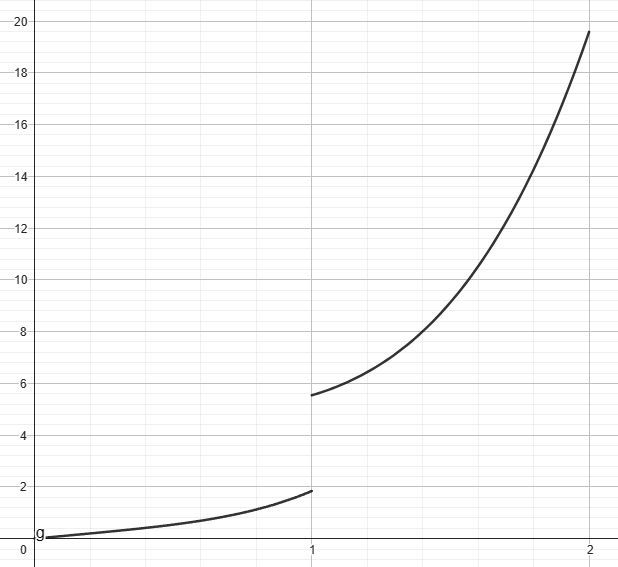
\includegraphics[width=7cm]{Images/figure_2/percobaanDua.png}
    \caption{Grafik fungsi $g$ pada eksperimen kedua}
    \label{grafikg2}
\end{figure}

Dari Gambar \ref{grafikg2} dapat dilihat bahwa fungsi $g$ tidak kontinu pada titik \mbox{$x=1$}. Eksperimen kedua dilakukan untuk mengamati tingkat akurasi metode ketika menginterpolasi fungsi yang tidak kontinu.

\subsection{Interval Sama Besar}
Dibentuk titik-titik pada interval $[0,2]$ berupa $x_j^l = j/2^l, ~ j=0,\dots,2^{l+1}$, dengan $l$ suatu bilangan bulat positif yang sudah ditentukan. Interval yang dibentuk di antara titik-titik yang dibentuk memiliki interval yang sama besar yaitu $h = 2^{-l}$. Berikut adalah grafik dan plot dari galat yang diperoleh jika dipilih $l = 4$ sehingga intervalnya sama besar yaitu $h=0.625$. 

Pada experimen titik-titik yang estimasi turunan pertamanya ditentukan dengan menggunakan metode nonlinear pada metode $\textbf{O}$ adalah titik-titik pada indeks $\{2^l-1, 2^l, 2^l+1, 2^l+2\}$ sedangkan pada metode $\textbf{R}$ titik-titik yang ditentukan estimasi turunan pertamanya menggunakan metode nonlinear adalah titik-titik pada indeks $\{2^l, 2^l+1\}$. Titik ini dipilih untuk mengamati perubahan nilai akurasi yang diperoleh dari kedua metode apabila panjang interval berubah-ubah.

\begin{figure}[H]
    \centering
    \raisebox{1.5cm}{\rotatebox[origin=t]{90}{$\textbf{S}$}}
    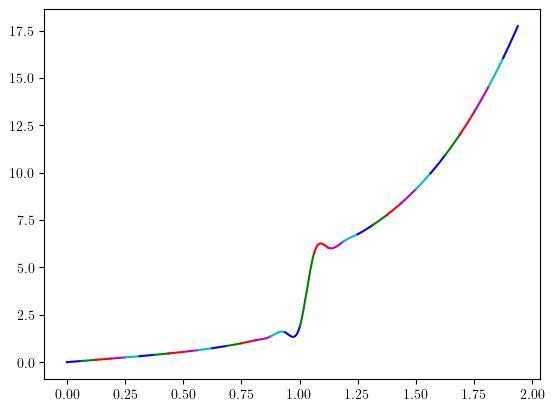
\includegraphics[width=5cm]{Images/figure_2/grafikS2.png}
    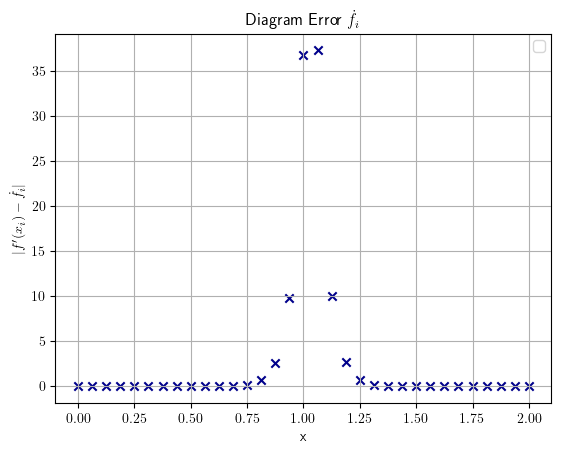
\includegraphics[width=5cm]{Images/figure_2/plotS2.png}
\end{figure}

\begin{figure}[H]
    \centering
    \raisebox{1.5cm}{\rotatebox[origin=t]{90}{$\textbf{O}_{FB}$}}
    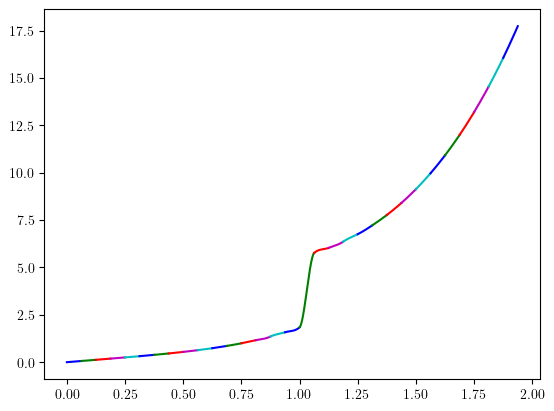
\includegraphics[width=5cm]{Images/figure_2/grafikOFB2.png}
    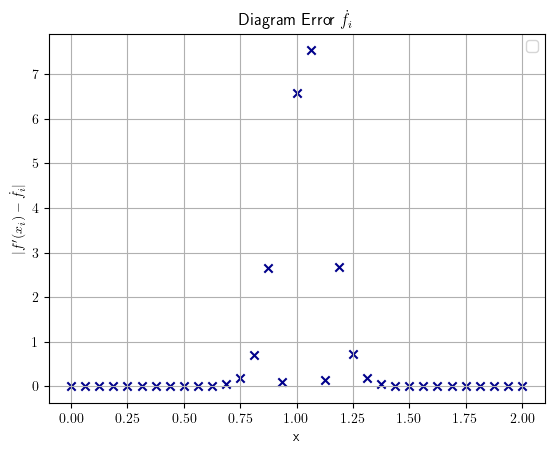
\includegraphics[width=5cm]{Images/figure_2/plotOFB2.png}
    \\
    \raisebox{1.5cm}{\rotatebox[origin=t]{90}{$\textbf{O}_{AY}$}}
    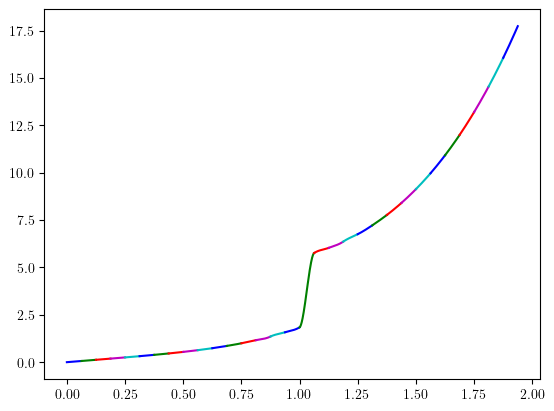
\includegraphics[width=5cm]{Images/figure_2/grafikOAY2.png}
    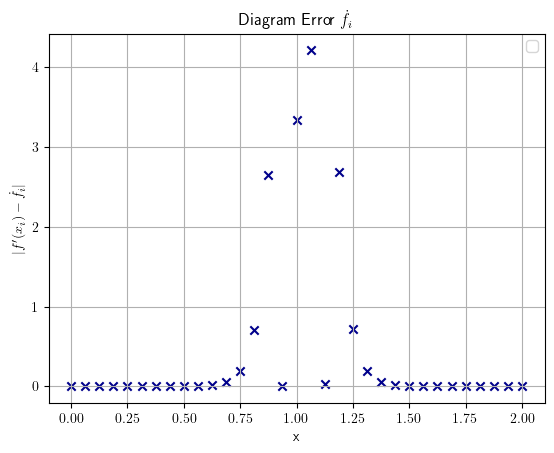
\includegraphics[width=5cm]{Images/figure_2/plotOAY2.png}
    \\
    \raisebox{1.5cm}{\rotatebox[origin=t]{90}{$\textbf{R}_{FB}$}}
    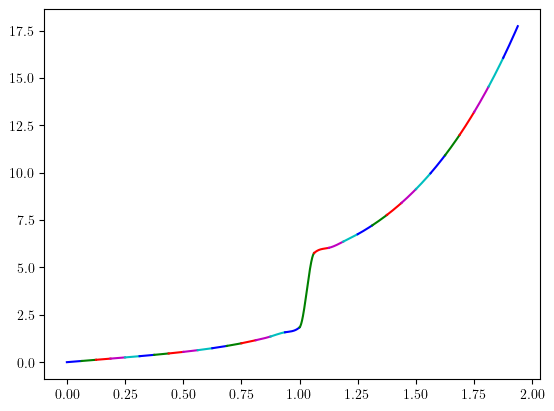
\includegraphics[width=5cm]{Images/figure_2/grafikRFB2.png}
    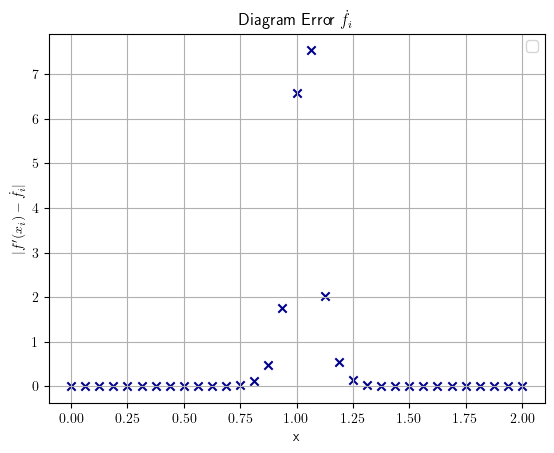
\includegraphics[width=5cm]{Images/figure_2/plotRFB2.png}
    \\
    \raisebox{1.5cm}{\rotatebox[origin=t]{90}{$\textbf{R}_{AY}$}}
    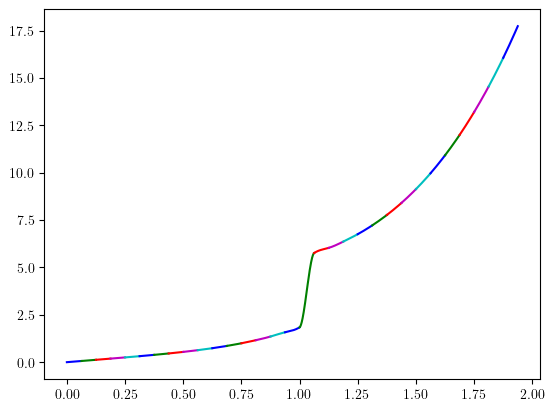
\includegraphics[width=5cm]{Images/figure_2/grafikRAY2.png}
    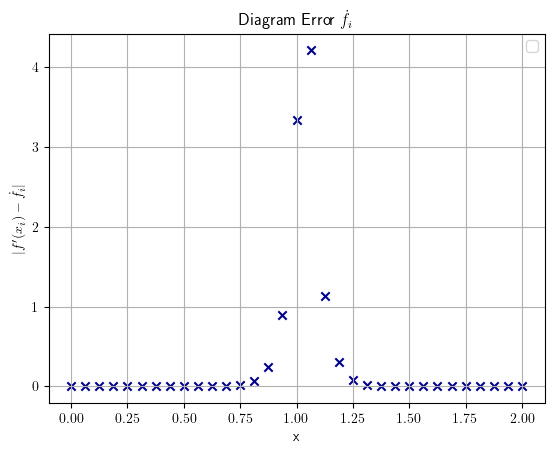
\includegraphics[width=5cm]{Images/figure_2/plotRAY2.png}
    \caption{Eksperimen kedua dengan $l=4$ interval sama besar}
    \label{grafikPlot2}
\end{figure}

    Pada Gambar \eqref{grafikPlot2} terlihat metode $\textbf{O}$ dan $\textbf{R}$ masing-masing menghasilkan hasil interpolasi yang monoton pada interval disekitar titik $x=1$ sedangkan metode $\textbf{S}$ mengalami osilasi pada hasil interpolasi saat mendekati titik $x=1$ di mana fungsi yang diinterpolasi tidak kontinu menyebabkan syarat monotonnya tidak terpenuhi. Selain itu galat dari hasil pendekatan turunan pertama yang dihasilkan dengan metode $\textbf{S}$ relatif sangat besar ketika mendekati titik $x=1$ dibandingkan dengan metode yang lainnya. Dapat dilihat juga galat yang diperoleh ketiga menggunakan metode nonlinear $FB$ menghasilkan galat yang lebih besar hingga dua kali galat ketika menggunakan metode $AY$.

    Perlu diperhatikan bahwa untuk eksperimen kedua pada titik $i_0 = 2^l$ syarat monoton selalu tidak terpenuhi karena pada titik fungsi yang diinterpolasi tidak kontinu pada interval $[x_{2^{l}}, x_{2^l + 1}]$. Berdasarkan Proposisi \ref{prpsslast} dengan $r=1$ didefinisikan himpunan indeks
    $$W=\{ i : 1\leq i \leq l_0 \text{ atau } l_1 \leq i \leq 2^{l+1} - 1\},$$ 
    dengan
    \begin{align*}
        l_0 = (i_0 - 1) + \log_2(\hat{h}) = (2^l - 1) + \log_2(2^{-l}) = 2^l - l - 1,\\
        l_1 = (i_0 + 1) - \log_2(\hat{h}) = (2^l + 1) - \log_2(2^{-l}) = 2^l + l + 2,
    \end{align*}
    berakibat diperoleh tabel estimasi order akurasinya sebagai berikut.

    \begin{table}[htp]
        \centering
        \resizebox{16cm}{!}{\begin{tabular}{|c|c|c|c|c|c|}
    \hline h&$\textbf{S}$&$\textbf{O}_{FB}$&$\textbf{O}_{AY}$&$\textbf{R}_{FB}$&$\textbf{R}_{AY}$ \\ 
    \hline
0.03125&0.896372535576625&0.896372535576625&0.896372535576625&2.9661347200468837&3.945353043785682 \\
0.015625&0.8981807720392228&0.8981807720392228&0.8981807720392228&2.934978479747872&3.925153321202357 \\
0.0078125&0.8990766668112026&0.8990766668112026&0.8990766668112026&2.918177295769085&3.91032575666795 \\
0.00390625&0.8995232015410665&0.8995232015410665&0.8995232015410665&2.9091723530199505&3.9071945357648943 \\
    \hline
    \end{tabular}}
        \caption{Tabel estimasi order akurasi eksperimen kedua dengan interval sama besar $h=2^{-l}$, $5 \leq l \leq 8$, $W=\{ i : 1\leq i \leq l_0 $ atau $l_1 \leq i \leq 2^{l+1}- 1\}$, $l_0 = 2^l - l - 1$ dan $l_1 =  2^l + l + 2$}
        \label{tabel7}
    \end{table}

    Dari Tabel \ref{tabel7} dapat disimpulkan bahwa metode $\textbf{O}$ mengalami penurunan akurasi lebih besar dari pada metode $\textbf{R}$ pada area disekitar $[x_{2^{l}}, x_{2^l+1}]$. Seperti sebelumnya dengan memanfaatkan Proposisi \ref{prpsslast} dan $r=2$ dibentuk himpunan yang lebih kecil berupa 
    $$W=\{ i : 1\leq i \leq l_0 \text{ atau } l_1 \leq i \leq 2^{l+1} - 1\},$$ 
    dengan
    \begin{align*}
        l_0 = (i_0 - 1) + 2\log_2(\hat{h}) = (2^l - 1) + 2\log_2(2^{-l}) = 2^l - 2l - 1,\\
        l_1 = (i_0 + 1) - 2\log_2(\hat{h}) = (2^l + 1) - 2\log_2(2^{-l}) = 2^l + 2l + 2,
    \end{align*}
    sehingga diperoleh estimasi order akurasi pada area tersebut pada tabel berikut.
    
    \begin{table}[htp]
        \centering
        \resizebox{16cm}{!}{\begin{tabular}{|c|c|c|c|c|c|}
    \hline h&$\textbf{S}$&$\textbf{O}_{FB}$&$\textbf{O}_{AY}$&$\textbf{R}_{FB}$&$\textbf{R}_{AY}$ \\ 
    \hline
0.03125&2.7960799781563304&2.7960799781563304&2.7960799781563304&4.8390922004107555&6.043717175770229 \\
0.015625&2.798034660598472&2.798034660598472&2.798034660598472&4.793213617610702&4.457115286101313 \\
0.0078125&2.7989979341003295&2.7989979341003295&2.7989979341003295&4.750282195219751&3.999927133695036 \\
0.00390625&2.79947361166368&2.79947361166368&2.79947361166368&4.673930753027552&3.957318743784382 \\
    \hline
    \end{tabular}}
        \caption{Tabel estimasi order akurasi eksperimen kedua dengan interval sama besar $h=2^{-l}$, $5 \leq l \leq 8$, $W=\{ i : 1\leq i \leq l_0 $ atau $l_1 \leq i \leq 2^{l+1}- 1\}$, $l_0 = 2^l - 2l - 1$ dan $l_1 =  2^l + 2l + 2$}
        \label{tabel8}
    \end{table}

    Tabel \ref{tabel8} memberikan estimasi order akurasi pada area yang lebih jauh dari titik $x=1$ di mana titik tidak kontinu. Dari hasil yang diperoleh, metode $\textbf{S}$, metode $\textbf{O}$, dan metode $\textbf{R}$ menghasilkan order akurasi yang lebih baik semakin menjauhi titik $x=1$ di mana fungsi yang diinterpolasi mengalami ketidak kontinuan.
    
\subsection{Interval Tidak Sama Besar}

Sama seperti pembuatan subinterval yang tidak sama besar pada eksperimen pertama dibentuk titik-titik
\begin{align*}
    x_{2j}^l = 2^{-l}j,\\
    x_{2j + 1}^l = 2^{-l}\left(j + \frac{1}{4}\right),
\end{align*}
dengan $j = 0,~1,\dots,~2^{l+1}$ sehingga diperoleh untuk suatu bilangan bulat $l$ subinterva-subinterval yang terbentuk di antara titik-titiknya memiliki interval terbesar \mbox{$\hat{h} = \frac{3}{4}2^{-l}.$} Dengan mengambil $l=3$, maka diperoleh grafik hasil interpolasi dan plot galat turunan pertama disetiap titik berikut.

\begin{figure}[H]
    \centering
    \raisebox{1.5cm}{\rotatebox[origin=t]{90}{$\textbf{S}$}}
    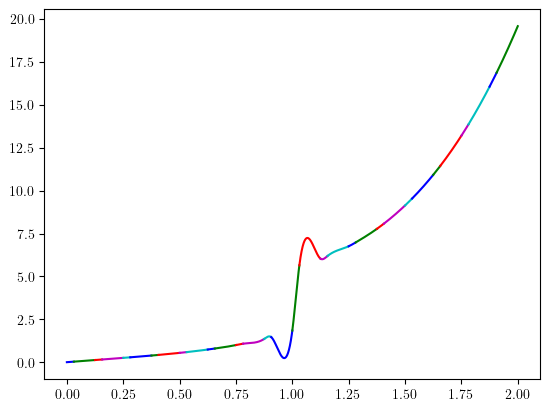
\includegraphics[width=6cm]{Images/figure_2/grafikS2n.png}
    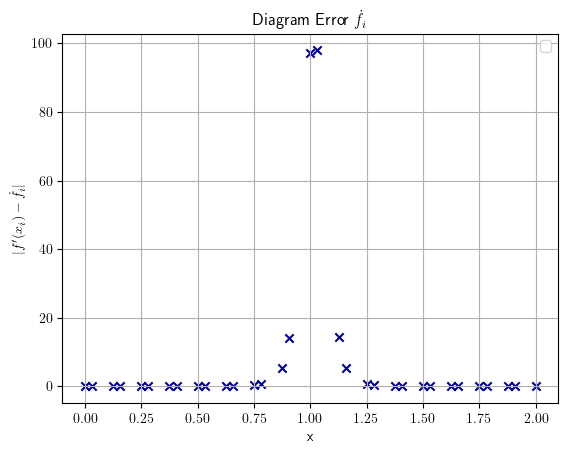
\includegraphics[width=6cm]{Images/figure_2/plotS2n.png}
\end{figure}

\begin{figure}[H]
    \centering
    \raisebox{1.5cm}{\rotatebox[origin=t]{90}{$\textbf{O}_{FB}$}}
    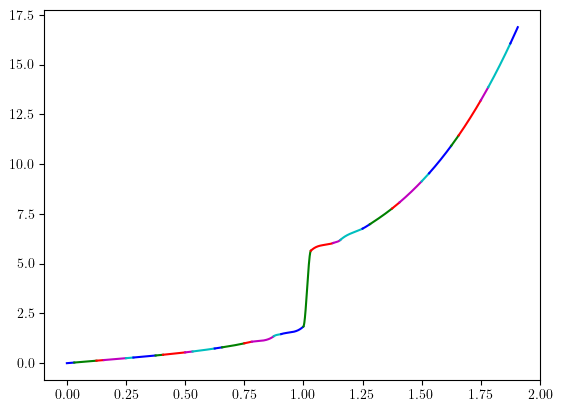
\includegraphics[width=6cm]{Images/figure_2/grafikOFB2n.png}
    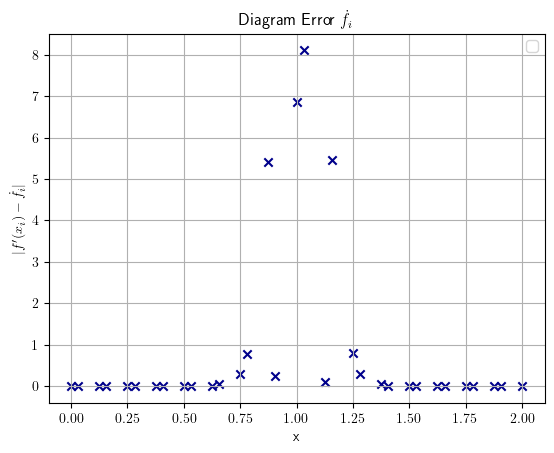
\includegraphics[width=6cm]{Images/figure_2/plotOFB2n.png}
    \\
    \raisebox{1.5cm}{\rotatebox[origin=t]{90}{$\textbf{O}_{AY}$}}
    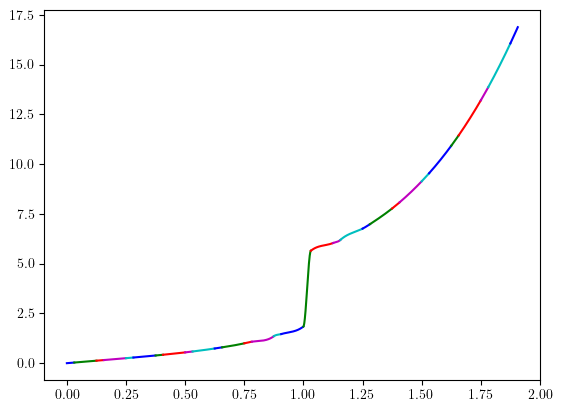
\includegraphics[width=6cm]{Images/figure_2/grafikOAY2n.png}
    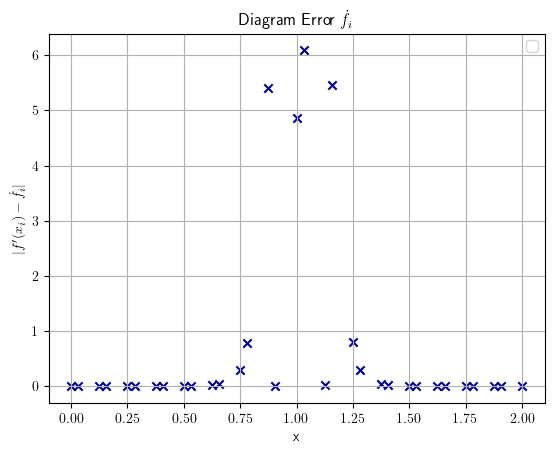
\includegraphics[width=6cm]{Images/figure_2/plotOAY2n.png}
    \\
    \raisebox{1.5cm}{\rotatebox[origin=t]{90}{$\textbf{R}_{FB}$}}
    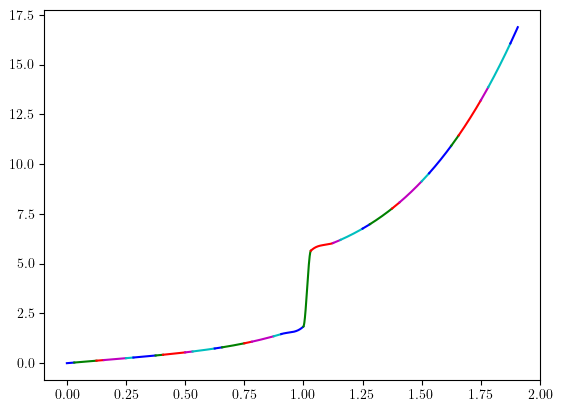
\includegraphics[width=6cm]{Images/figure_2/grafikRFB2n.png}
    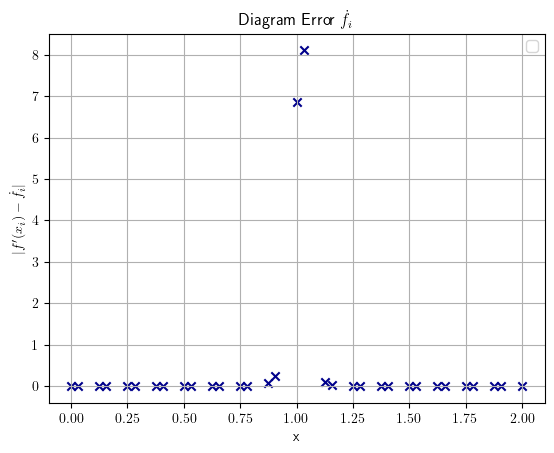
\includegraphics[width=6cm]{Images/figure_2/plotRFB2n.png}
    \\
    \raisebox{1.5cm}{\rotatebox[origin=t]{90}{$\textbf{R}_{AY}$}}
    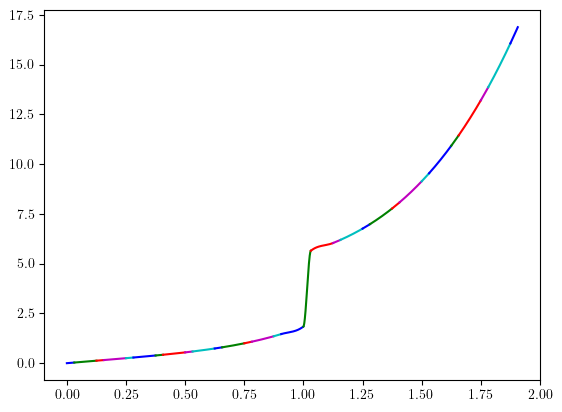
\includegraphics[width=6cm]{Images/figure_2/grafikRAY2n.png}
    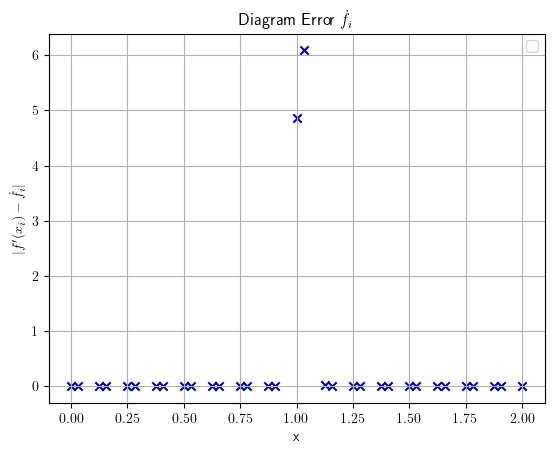
\includegraphics[width=6cm]{Images/figure_2/plotRAY2n.png}
    \caption{Eksperimen kedua dengan $l=4$ interval tidak sama besar}
    \label{grafikPlot2n}
\end{figure}

Gambar \eqref{grafikPlot2n} memberikan grafik fungsi interpolasi dan plot galat turunan dari setiap metode. Dari hasil plot tersebut dapat disimpulkan metode $\textbf{R}$ memberikan hasil pendekatan turunan pada sekitar titik tidak kontinu dengan galat yang paling kecil dibandingkan dengan metode lainnya.

Untuk mengamati order akurasi dari turunan pertama disekitar titik $x=1$ didefinisikan himpunan indeks
\begin{align*}
    W = \{ i: 0 \leq i \leq l_0 \text{ atau } l_1 \leq i \leq 2^{l+2} \},
\end{align*}
dengan
\begin{align*}
    l_0 = (i_0 - 1) + \log_2(\hat{h}) = (2^{l+1} - 1) + \log_2\left(\frac{3}{4} 2^{-l}\right), \\
    l_1 = (i_0 + 1) - \log_2(\hat{h}) = (2^{l+1} + 2) - \log_2\left(\frac{3}{4} 2^{-l}\right).
\end{align*}
Estimasi order akurasi yang digunakan sama seperti pada eksperimen pertama yaitu menggunakan
\begin{align*}
    \Tilde{o}_l^W := \log_4\left(\frac{e_{l}^W}{e_{l-2}^W}\right).
\end{align*}
Dengan mengamati titik-titik tersebut maka diperoleh hasil estimasi order akurasi sebagai berikut.

\begin{table}[htp]
        \centering
        \resizebox{16cm}{!}{\begin{tabular}{|c|c|c|c|c|c|}
    \hline h&$\textbf{S}$&$\textbf{O}_{FB}$&$\textbf{O}_{AY}$&$\textbf{R}_{FB}$&$\textbf{R}_{AY}$ \\ 
    \hline
0.0234375&1.0791206523482317&1.0791206523482317&1.0791206523482317&2.016816138147151&2.955130599603732 \\
0.005859375&1.0823271429167844&1.0823271429167844&1.0823271429167844&1.7387074723422433&3.024111952732935 \\
0.00146484375&1.0826615986711732&1.0826615986711732&1.0826615986711732&2.3353545234629536&2.9913528591017755 \\
    \hline
    \end{tabular}}
        \caption{Tabel estimasi order akurasi eksperimen kedua dengan interval tidak sama besar $\hat{h}=\frac{3}{4}2^{-l}$, $5 \leq l \leq 8$, $W=\{ i : 1\leq i \leq l_0 $ atau $l_1 \leq i \leq 2^{l+1}- 1\}$, $l_0 = (2^{l+1} - 1) + \log_2(\frac{3}{4}2^{-l})$ dan $l_1 = (2^{l+1} + 2) - \log_2(\frac{3}{4}2^{-l})$}
        \label{tabel9}
    \end{table}

Dari Tabel \ref{tabel9} hasil estimasi order akurasi masih belum menghasilkan hasil interpolasi yang optimal pada area sekitar titik yang tidak kontinuan, baik menggunakan metode $\textbf{S}$ dan metode $\textbf{O}$. Pada metode $\textbf{R}$ order akurasi terlihat meningkat, namun belum menghasilkan interpolasi yang optimal.

Selanjutnya akan diamati untuk titik-titik yang lebih jauh dari titik di mana fungsi $g$ tidak kontinu. Dibentuk
\begin{align*}
    W = \{ i: 0 \leq i \leq l_0 \text{ atau } l_1 \leq i \leq 2^{l+2} \},
\end{align*}
dengan
\begin{align*}
    l_0 = (i_0 - 1) + 2\log_2(\hat{h}) = (2^{l+1} - 1) + 2\log_2(\frac{3}{4} 2^{-l}), \\
    l_1 = (i_0 + 1) - 2\log_2(\hat{h}) = (2^{l+1} + 2) - 2\log_2(\frac{3}{4} 2^{-l}),
\end{align*}
sehingga diperoleh hasil estimasi order akurasi pada tabel berikut
\begin{table}[htp]
        \centering
        \resizebox{16cm}{!}{\begin{tabular}{|c|c|c|c|c|c|}
    \hline h&$\textbf{S}$&$\textbf{O}_{FB}$&$\textbf{O}_{AY}$&$\textbf{R}_{FB}$&$\textbf{R}_{AY}$ \\ 
    \hline
0.0234375&3.1292610123804017&3.1292610123804017&3.1292610123804017&2.986526501124396&2.995424643389291 \\
0.005859375&3.12741868305077&3.12741868305077&3.12741868305077&2.9972376302527652&2.9974828976530117 \\
0.00146484375&3.121560690369995&3.121560690369995&3.121560690369995&2.998864243982574&2.999072449078856\\
    \hline
    \end{tabular}}
        \caption{Tabel estimasi order akurasi eksperimen kedua dengan interval tidak sama besar $\hat{h}=\frac{3}{4}2^{-l}$, $5 \leq l \leq 8$, $W=\{ i : 1\leq i \leq l_0 $ atau $l_1 \leq i \leq 2^{l+1}- 1\}$, $l_0 = (2^{l+1} - 1) + 2\log_2(\frac{3}{4}2^{-l})$ dan $l_1 = (2^{l+1} + 2) - 2\log_2(\frac{3}{4}2^{-l})$}
        \label{tabel10}
    \end{table}

Dari Tabel \ref{tabel10}, diperoleh bahwa semua metode menghasilkan pendekatan dengan tingkat akurasi order ketiga. Hal ini mengindikasikan hasil interpolasi sudah optimal berdasarkan Lema \ref{orderAkurasi} untuk titik yang jauh dari titik tidak kontinu.

\section{Eksperimen Ketiga}

Untuk eksperimen ketiga akan dicoba menginterpolasi titik-titik yang sama dengan interpolasi spline kubik pada Subbab \textbf{3.1} yaitu $(0,10)$, $(1,8.7)$, $(2,2.1)$, $(3,1.5)$, dan $(4,0.1)$. Dengan metode interpolasi yang telah dibahas sebelumnya, maka diperoleh grafik hasil interpolasi berikut
\begin{figure}[H]
    \centering
    \raisebox{1.5cm}{\rotatebox[origin=t]{90}{$\textbf{S}$}}
    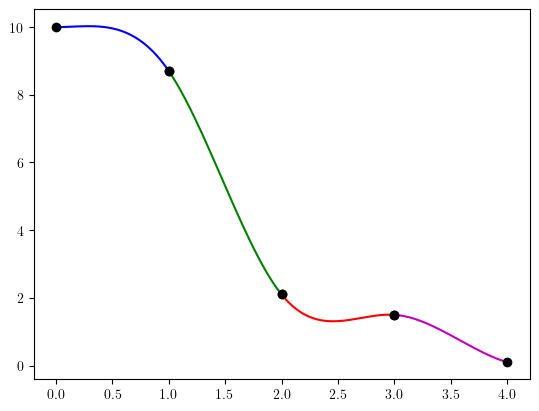
\includegraphics[width=8cm]{Images/figure_2/grafikS3.png}
\end{figure}

\begin{figure}[H]
    \centering
    \raisebox{1.5cm}{\rotatebox[origin=t]{90}{$\textbf{O}_{FB}$}}
    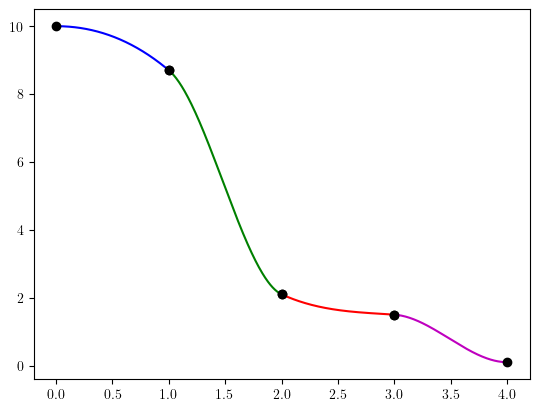
\includegraphics[width=8cm]{Images/figure_2/grafikOFB3.png}
    \\
    \raisebox{1.5cm}{\rotatebox[origin=t]{90}{$\textbf{O}_{AY}$}}
    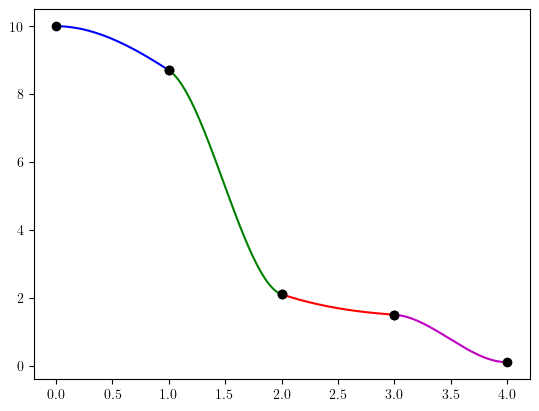
\includegraphics[width=8cm]{Images/figure_2/grafikOAY3.png}
    \\
    \raisebox{1.5cm}{\rotatebox[origin=t]{90}{$\textbf{R}_{FB}$}}
    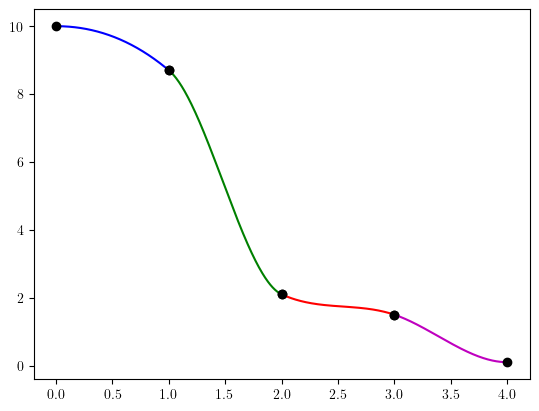
\includegraphics[width=8cm]{Images/figure_2/grafikRFB3.png}
    \\
    \raisebox{1.5cm}{\rotatebox[origin=t]{90}{$\textbf{R}_{AY}$}}
    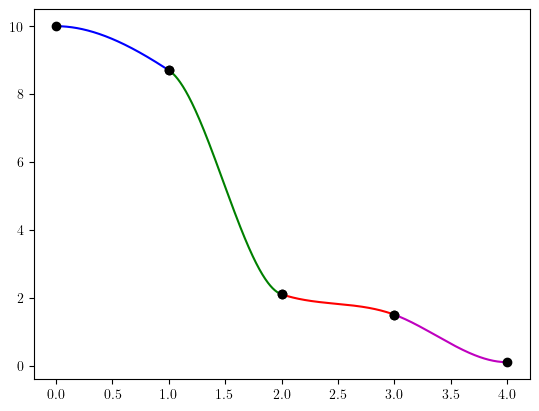
\includegraphics[width=8cm]{Images/figure_2/grafikRAY3.png}
    \caption{Eksperimen ketiga menginterpolasi titik-titik yang diberikan}
    \label{grafikPlot3}
\end{figure}

Dari Gambar \ref{grafikPlot3} diperoleh hasil interpolasi yang diperoleh monoton. Berbeda dengan hasil interpolasi sebelumnya, hasil interpolasi yang dihasilkan memiliki sifat monoton. Karena data yang diinterpolasi memiliki sifat monoton, maka hasil interpolasi yang diharapkan juga harus monoton. Hasil interpolasi yang monoton menyebabkan data hasil interpolasi yang diperoleh menjadi lebih akurat.